\documentclass{article}
\usepackage[utf8]{inputenc}
\usepackage{amsmath}
\usepackage{graphicx}
\usepackage{BeginnerStyleFile}
\graphicspath{ {images/} }

\title{Reading Summary 4.2}
\author{Evan Hughes}
\date{March 2023}

\begin{document}
\maketitle
\section*{4.3 Irreducibles and Unique Factorization}
Throughout these sections $F$ has always been a field. Before carrying over the results
of section 1.3 on unique factorization in $\mathbb{Z}$ to the ring of polynomials over a field,
we must first examine an area in which $\mathbb{Z}$ differs significantly from $F[x]$.
In $\mathbb{Z}$ there are only two units, $\pm 1$, but a polynomial ring may have
many more units.

An element $a$ in a commutative ring with identity $R$ is said to be an associate of an element $b$
of $R$ if $a=bu$ for some unit $u$. In this case $b$ is also an associate of $a$ because $u^-1$ is a unit and $b = au^-1$.
In the ring $\mathbb{Z}$, the only associates of an integer $n$ are $n$ and $-n$ because
$\pm 1$ are the only units. If $F$ is a field, then by Corollary 4.5, the units in $F[x]$ are the
nonzero constants. Therefore, $f(x)$ is an associate of $g(x)$ in $F[x]$ if and only if $f(x) = cg(x)$ for some nonzero $c\in F$.


\subsection*{Definition}

Let $F$ be a field. A nonconstant polynomial $p(x) \in F[x]$ is said
to be irreducible if its only divisors are its associates and the nonzero constant polynomials. A nonconstant polynomial
that is not irreducible is said to be reducible. 

\subsection*{Example (from the book)}

The polynomial $x+2$ is irreducible in $\mathbb{Q}[x]$ because
all its divisors must have degree 0 or 1. Divisors of degree 0 are nonzero constants.
$f(x)\mid (x+2)$, say $x+2 = f(x)g(x)$, and if deg$f(x)=1$, then $g(x)$ has degree $0$, so that $g(x) = c$.
Thus $c^-1(x+2) = f(x)$, and $f(x)$ is an associate of $x+2$.
A similar argument in the general case shows that \textbf{every polynomial of degree $1$ in $F[x]$ is irreducible in $F[x]$}.

\subsection*{Theorem 4.11}
Let $F$ be a field. A nonzero polynomial $f(x)$ is reducible in $F[x]$ if 
and only if $f(x)$ can be written as the product of two polynomials of lower degree.

\subsection*{Proof}
First assume that $f(x)$ is reducible. Then it must have a divisor $g(x)$
that is neither an associate nor a nonzero constant, say $f(x) = g(x)h(x)$.
If either $g(x)$ or $h(x)$ has the same degree as $f(x)$, then the other must have degree $0$.
Since a polynomial of drgee $0$ is a nonzero constant in $F$, this means 
that either $g(x)$ is a constant or an associate $f(x)$, contrary to the hypothesis.
Therefore, both $g(x)$ and $h(x)$ have lower degree than $f(x)$.

Now assume that $f(x)$ can be written as the product of two polynomials of lower degree.
That means $f(x) = g(x)h(x)$ with both $g(x)$ and $h(x)$ having lower degree than $f(x)$.
Which means that $f(x)$ has a divisor that is neither an associate nor a nonzero constant. $\blacksquare$

\subsection*{Theorem 4.12}
Let $F$ be a field and $p(x)$ a nonconstant polynomial in $F[x]$.
Then the following conditions are equivalent:
\begin{enumerate}
    \item $p(x)$ is irreducible.
    \item If $b(x)$ and $c(x)$ are any polynomials such that $p(x)\mid b(x)c(x)$, then
    $p(x)\mid b(x)$ or $p(x)\mid c(x)$.
    \item If $r(x)$ and $s(x)$ are any polynomials such that $p(x)=r(x)s(x)$, then $r(x)$ or $s(x)$ is a nonzero constant polynomials.
\end{enumerate}

\subsection*{Proof}
$(1) \implies (2)$ Adapt the proof of Theorem 1.5 to $F[x]$.
Replace statements about $\pm p$ by statements about the associates of $p(x)$;
replace statements about $\pm 1$ by statements about the nonzero constants in $F[x]$(units).
Use Theorem 4.10 in place of Theorem 1.4.

\vspace*{5mm}
$(2) \implies (3)$ If $p(x) = r(x)s(x)$, then $p(x)\mid r(x)$ or
$p(x)\mid s(x)$ by $(2)$. If $p(x)\mid r(x)$, say $r(x) = p(x)q(x)$,
then $p(x)=r(x)s(x) = p(x)v(x)s(x)$. Since $F[x]$ is and i.d.
we can cancel $p(x)$ by Theorem 3.7 and conclude that $1_F = v(x)s(x)$.
This $s(x)$ is a unit, and hence by Corollary 4.5, $s(x)$ is a nonzero constant.
A similar argument shows that if $p(x)\mid s(x)$, then $r(x)$ is a nonzero constant.

\vspace*{5mm}
$(3) \implies (1)$ Let $c(x)$ be any divisor of $p(x)$, say $p(x) = c(x)d(x)$.
Then by $(3)$, either $c(x)$ or $d(x)$ is a nonzero constant.
If $d(x) = d \neq 0_p$, then multiplying both sides of
$p(x) = c(x)d(x) = dc(x)$ by $d^{-1}$ shows that $c(x) = d^{-1}p(x)$.
Thus in every case, $c(x)$ is a nonzero constant or an 
associate of $p(x)$. Therefore, $p(x)$ is irreducible. $\blacksquare$

\subsection*{Corollary 4.13}
Let $F$ be a field and $p(x)$ an irreducible polynomial in $F[x]$.
If $p(x)\mid a_1(x)a_2(x)\cdots a_n(x)$, then $p(x)$ divides at least on of the $a_i(x)$.
To prove adapt the proof of Corollary 1.6 to $F[x]$. $\blacksquare$ 

\subsection*{Theorem 4.14}
Let $F$ be a field. Every nonconstant polynomial $f(x)$ in $F[x]$ is a product of irreducible polynomials 
in $F[x]$(We allow the possibility of a product with just one factor incase $f(x)$ is itself irreducible).
This factorization is unique in the following sense: If
\begin{center}
    $f(x) = p_1(x)p_2(x)\cdots p_k(x)$ and $f(x) = q_1(x)q_2(x)\cdots q_k(x)$
\end{center}

with each $p_i(x)$ and $q_i(x)$ irreducible, then $r = s$(that is,
the number of irreducible factors is the same). After the $q_i(x)$
are reordered and relabeled, if necessary,
\begin{center}
    $p_i(x)$ is an associate of $q_i(x)$ \, $(i = 1,2,3\cdots,r)$.
\end{center}

\subsection*{Proof}
To show that $f(x)$ is a product of irreducibles, adapt the proof of Theorem 1.7
to $F[x]$: Let $S$ be the set of all nonconstant polynomials that are not the product
of irreducibles, and use a proof by contradiction to show that $S$ is empty.
To prove that this factorization is unique up to associates, suppose
$f(x) = p_1(x)p_2(x)\cdots p_i(x) = q_1(x)q_2(x)\cdots q_j(x)$ with each
$p_i(x)$ and $q_j(x)$ irreducible. Then $p_1(x)[p_2(x)\cdots p_i(x)] = q_1(x)q_2(x)\cdots q_j(x)$
so that $p_1(x)$ divides $q_1(x)q_2(x)\cdots q_j(x)$. Corollary 4.13 shows that
$p_i(x) \mid q_j(x)$ for some $j$. After rearranging and relabeling the $q(x)$'s
if necessary, we may assume that $p_1(x)\mid q_1(x)$. Since $q_1(x)$ is irreducible,
$p_1(x)$ must be either a constant or an associate of $q_1(x)$. However, 
$p_1(x)$ is irreducible, and so its not a constant. Therefore, $p_1(x)$ is an 
associate of $q_1(x)$, with $p_1(x) = c_1q_1(x)$ for some constant $c_1$. Thus
\begin{center}
    $q_1(x)[c_1p_2(x)p_3(x)\cdots p_i(x)] = p_1(x)p_2(x)\cdots p_r(x) = q_1(x)q_2(x)\cdots q_j(x)$.
\end{center}

Canceling $q_1(x)$ on each end, we have
\begin{center}
    $p_2(x)[c_1p_3(x)\cdots p_i(x)] = q_2(x)q_3(x)\cdots q_j(x)$.
\end{center}

Complete the argument by adapting the proof of Theorem 1.8 to $F[x]$,
replacing statements about $\pm q_j$ with statements about associates of $q_j(x)$. 
$\blacksquare$

\subsection*{Example(Exercise 3)}
$(3)$ List all associates of $x^2 + x + 1$ in $\mathbb{Z}_5[x]$.
\begin{enumerate}
    \item $a(x) = 1(x^2 + x + 1)$
    \item $b(x) = 2(x^2 + x + 1)$
    \item $c(x) = 3(x^2 + x + 1)$
    \item $d(x) = 4(x^2 + x + 1)$
\end{enumerate}




\begin{figure}
    \centering
    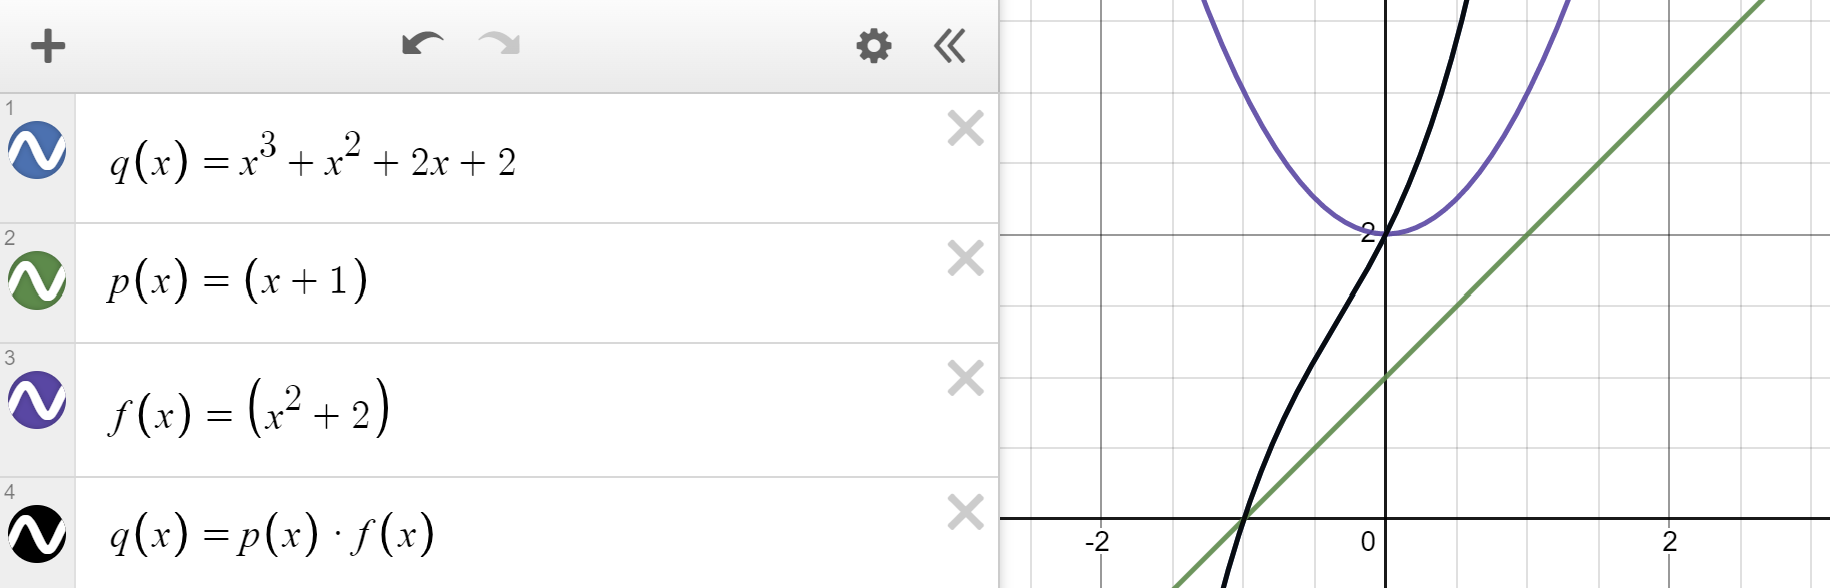
\includegraphics[width=0.6\textwidth]{factoredpolynomials.png}
    \caption{Factored polynomials in $\mathbb{Z}[x]$. While $x^3 + x^2 + 2x + 2$ can be reduced, one of its factors $x^2 + 2$ is irreducible in $\mathbb{Z}[x]$}
    \label{fig:division_algorithm}
\end{figure}


\end{document}